\chapter{Introduction}\label{sec:intro}

\section{Motivation}\label{sec:intro_motivation}
\begin{marginfigure}[1in]
    \centering
	\begin{subfigure}[b]{\textwidth}
    	\centering
        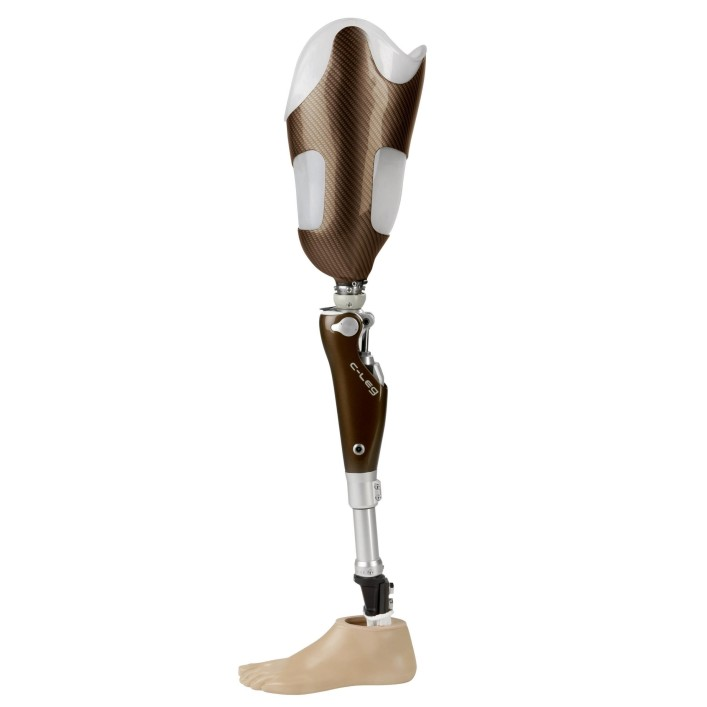
\includegraphics[height=1.5in]{ottobock_cleg}
        \caption{C-Leg™ Knee ©Ottobock}
        \label{fig:ottobock_cleg}
        \vspace{0.25in}
	\end{subfigure}
	\begin{subfigure}[b]{\textwidth}
    	\centering
        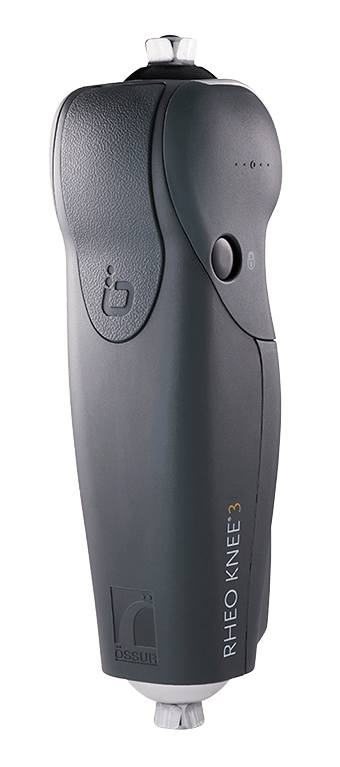
\includegraphics[height=1.5in]{rheo-knee}
        \caption{Rheo™  Knee ©Össur}
        \label{fig:ossur_rheo}
        \vspace{0.25in}
	\end{subfigure}
	\begin{subfigure}[b]{\textwidth}
    	\centering
        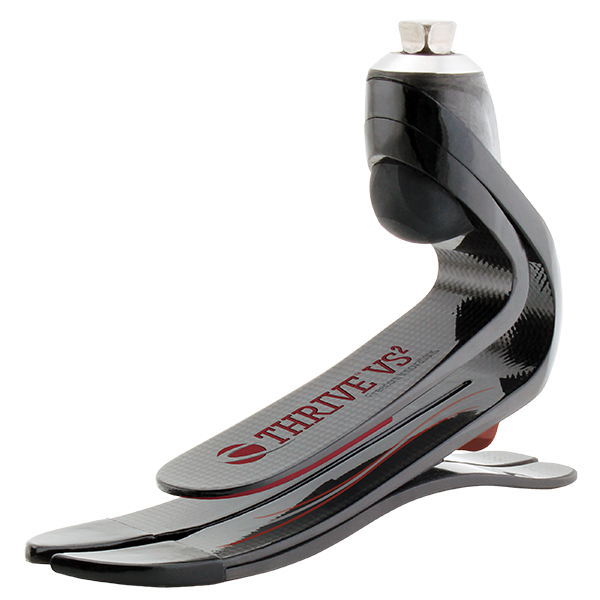
\includegraphics[height=1.5in]{freedom_innov_foot}
        \caption{Thrive™ Foot ©Freedom Innovations}
        \label{fig:freedom_innovations_foot}
	\end{subfigure}
    \caption{Examples of microprocessor-controlled mechanically-passive knee
    prostheses (a,b) and a energy storage and return ankle-foot prosthesis (c).}
\end{marginfigure}
\newthought{Six hundred thousand} lower-limb amputees currently live in the
United States according to recent estimates \citep{ziegler2008estimating}.
People undergo amputations due to a variety of reasons including traumatic
injuries from workplace accidents, traffic collisions, and as casualties of war.
In addition, a large percentage (54\%) suffer from the loss of a limb due to
complications arising from dysvascular disease associated with diabetes.
Consequently, largely due to the expected increase in diabetes in the coming
years, \citet{ziegler2008estimating} estimate that by 2050 the number of
amputees living in the United States will likely double.

Currently, prosthetists often prescribe transfemoral amputees (those with
amputations between the hip and knee joints) an energy storage and return
composite foot such as the Thrive Foot (Freedom Innovations; Irvine, CA;
\cref{fig:freedom_innovations_foot}) along with a microprocessor-controlled,
mechanically-passive knee prosthesis. These knee prostheses feature control
algorithms that adjust the knee's resistance in response to kinematic and force
data measured by sensors embedded in the device. Examples of
microprocessor-controlled prosthetic knees include the C-Leg (Otto Bock;
Duderstadt, Germany; \cref{fig:ottobock_cleg}), which has an adjustable
hydraulic damping system, and the Rheo Knee (Össur; Reykjavik, Iceland;
\cref{fig:ossur_rheo}), which achieves variable damping via a magnetorheological
fluid. While \citet{johansson2005clinical} show these microprocessor-controlled
knees can improve amputee gait characteristics by decreasing metabolic energy
consumption and peak hip torque and increasing gait smoothness compared to that
provided by fully-passive knee prosthesis, these prostheses still cannot fully
replicate healthy leg behavior as they are incapable of providing positive power
during the gait cycle. 

Positive power at the knee is evident in a number of locomotion tasks including
level walking \citep{perry2010gait}, walking up stairs
\citep{nadeau2003frontal}, running \citep{buczek1990stance}, and jumping
\citep{hubley1983work}. In addition, active knee flexion and extension muscle
activations have been noted during stumble recovery \citep{eng1994strategies}.
At the ankle joint, passive spring-like prostheses cannot replicate the positive
net work seen in the ankle joint during level ground walking, which is essential
for push-off and forward propulsion \citep{perry2010gait}.

Consequently, lower-limb amputees and especially \emph{transfemoral amputees},
those with above the knee amputations, equipped with mechanically-passive
prostheses suffer from a number of issues including markedly increased energy
consumption~\citep{waters1976energy}, abnormal gait
kinematics~\citep{jaegers1995prosthetic}, and an increased likelihood of
falling~\citep{miller2001prevalence}. Specifically, large percentages of
transfemoral amputees report they are unable to complete tasks such as walking
outside in inclement weather (47.4\%), walking while carrying a load (42.7\%),
walking up or down stairs without a handrail (38.5\%, 37.9\%), walking outside
on uneven terrain (29.5\%), picking up an object from the ground (28.1\%) or
getting up from the floor after a fall (22.8\%) \citep{gauthier1999enabling}.

Importantly, these gait pathologies can lead to an avoidance of walking
\citep{gauthier1999enabling}. This is especially true in the case of falls.
\citet{miller2001prevalence} find 49.2\% of lower limb amputees feared falling
and that of those afraid of falls 76\% avoided physical activity as a result.
Avoidance of physical activity is eminently concerning as it may lead to reduced
strength, endurance, and balance, feeding a positive feedback loop that causes
further debilitation.
\begin{figure*}[b]
    \centering
	\begin{subfigure}[b]{0.3\textwidth}
    	\centering
        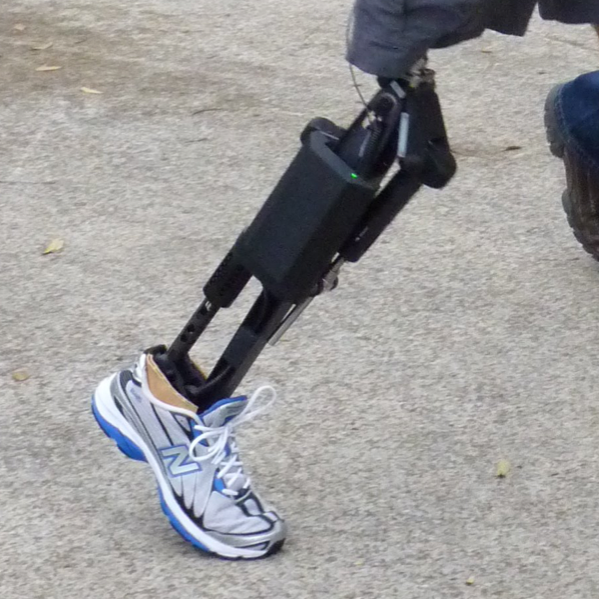
\includegraphics[width=2in]{VU_gen_1}
        \caption{Generation 1}
	\end{subfigure}
	\begin{subfigure}[b]{0.3\textwidth}
    	\centering
        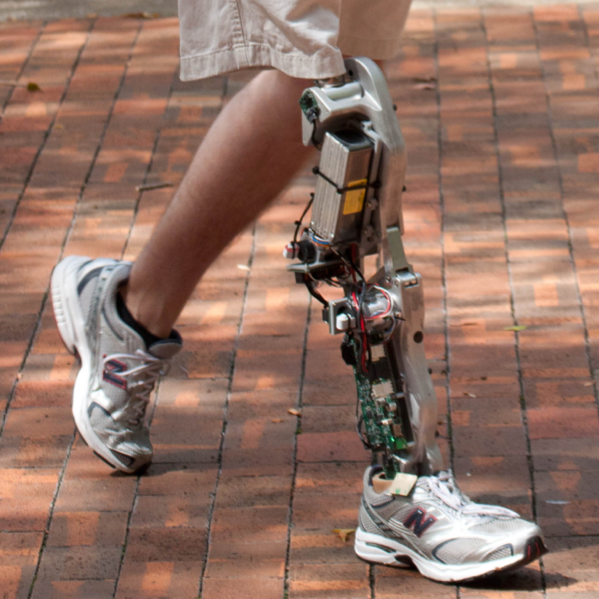
\includegraphics[width=2in]{VU_gen_2}
        \caption{Generation 2}
	\end{subfigure}
	\begin{subfigure}[b]{0.3\textwidth}
    	\centering
        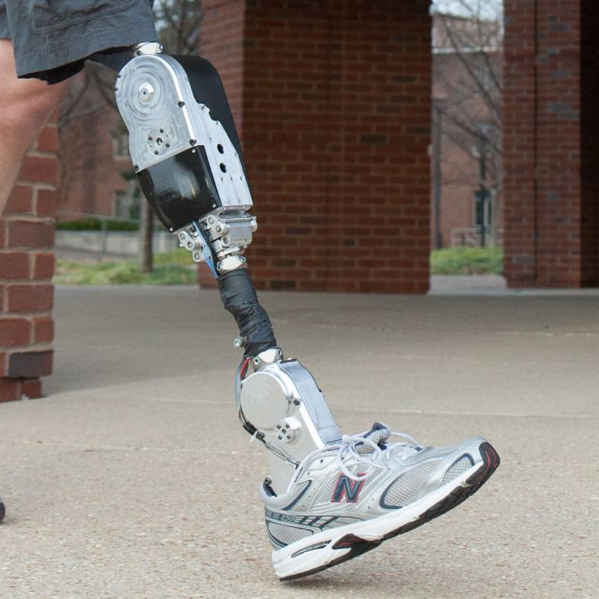
\includegraphics[width=2in]{VU_gen_3}
        \caption{Generation 3}
	\end{subfigure}
    \caption{Vanderbilt University's Robotic Transfemoral
    Prostheses. Images courtesy of Michael Goldfarb.\vspace{0.1in}}
    \label{fig:vanderbilt_prostheses_intro}
\end{figure*}

To help remedy this situation, in the past decade academic research groups and
companies have developed robotic powered knee and ankle prostheses for
lower-limb amputees.  These prostheses feature actuators at the knee and/or
ankle that, if controlled correctly, could potentially restore the kinetics,
kinematics, and reactions of the healthy human leg. Notable examples include
three generations of transfemoral prostheses developed by Vanderbilt
University~(\cref{fig:vanderbilt_prostheses_intro}) \citep{sup2009preliminary,
lawson2013control, lawson2014robotic} and the Biom powered
ankle~(\cref{fig:biom_ankle}) \citep{herr2012bionic}. These powered prostheses
have helped amputees walk on level ground more naturally and efficiently, as
well as walk up stairs and slopes \citep{sup2011upslope, lawson2013control}, run
\citep{huff2012running, shultz2015running}, perform sit-to-stand
\citep{varol2009powered}, and dance \citep{rouse2015design}. These results
illustrate the benefits of powered prostheses as many of these tasks require
positive joint power and thus would be difficult to perform with
mechanically-passive prostheses.

\begin{marginfigure}[-1in]
    \centering
    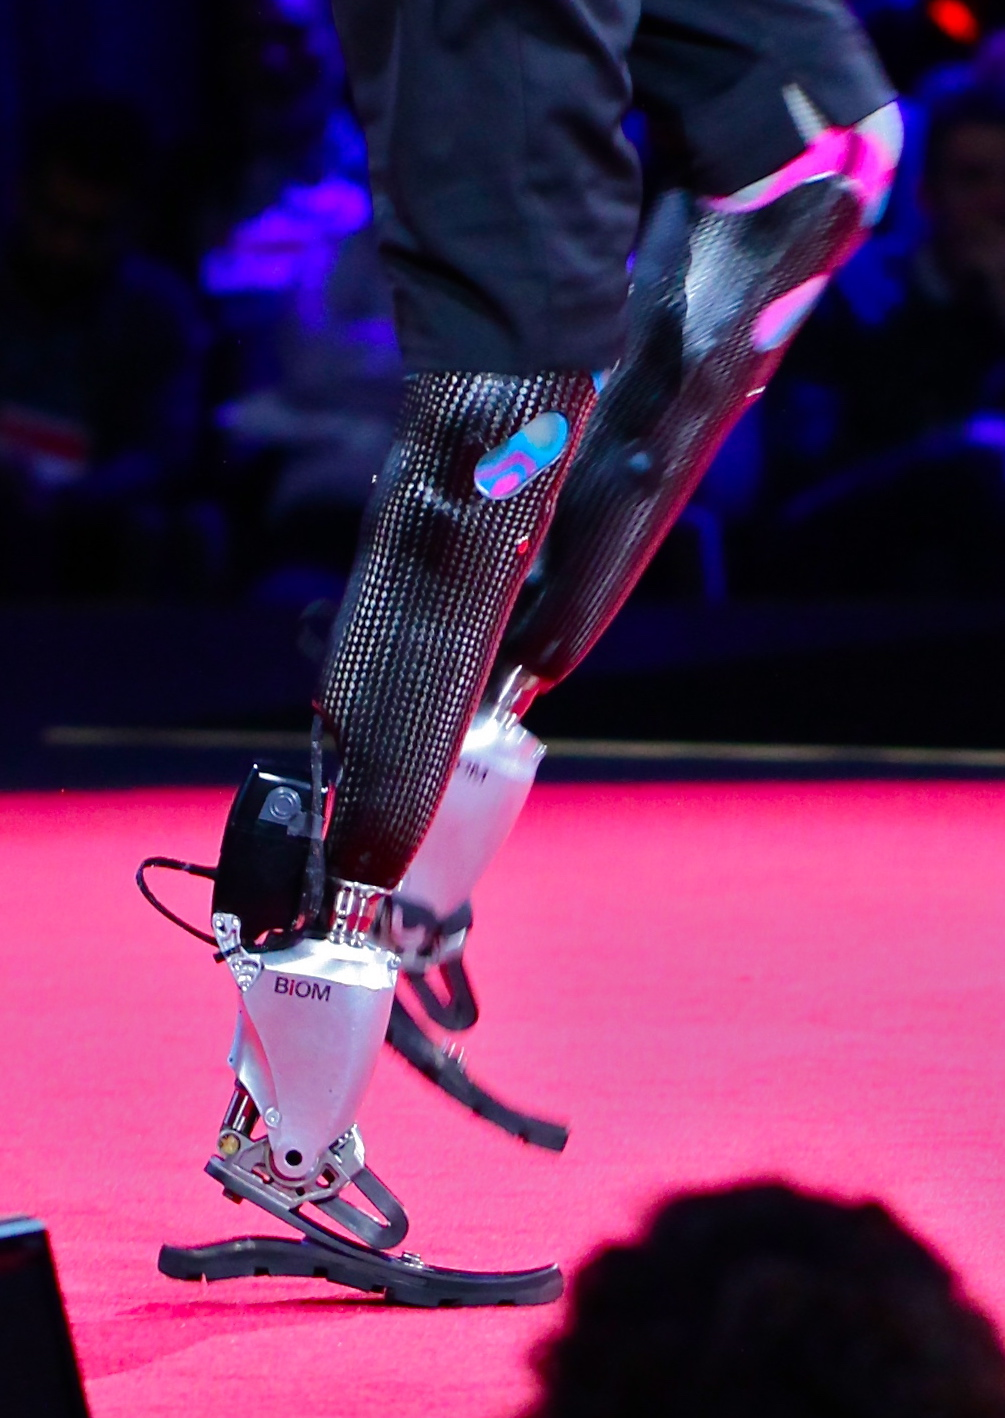
\includegraphics[width=\linewidth]{biom_prosthesis}
    \caption{Biom Robotic Ankle Prosthesis. Photo by
    \href{https://www.flickr.com/photos/jurvetson/13480667874/}{Steve
    Jurvetson}, \href{http://creativecommons.org/licenses/by/2.0}{CC BY 2.0},
    \href{https://commons.wikimedia.org/w/index.php?curid=32568854}{Link}
    (cropped from original).}
    \label{fig:biom_ankle}
\end{marginfigure}

\section{Challenges in Transfemoral Prosthesis
Control}\label{sec:intro_challenges} 

It still remains an open research question how best to control these prostheses
to achieve natural and robust gaits. In the most established control method for
powered prostheses, the prosthesis uses simple functions to approximate the
joint torque versus angle relationship, termed the \emph{quasi-stiffness}
observed during walking~\citep{sup2007design, lenzi2014speed}. However, since
the torque functions only approximate steady, level walking, this method
requires further tuning to handle other situations such as walking on
slopes~\citep{sup2011upslope} or rough ground~\citep{thatte2016toward} and
changing foot placement targets~\citep{schepelmann2016evaluation}. 

As mentioned earlier, walking on slopes and rough ground present major hurdles
for transfemoral amputees. Moreover, previously developed prosthesis controls
have not specifically addressed the risk of falling that is so detrimental to
amputee quality of life. Therefore, it is clear that we should formulate a
prosthesis controller with more power to generalize to a larger variety of
environments, which will improve amputee gait robustness. Formulating a robotic
prosthesis controller to accomplish this goal requires we address three main
challenges:

\begin{challenges}
    \item\label{chal:dynamic} \emph{Human locomotion is a dynamic task}~~During
    stance, the leg acts in a compliant, spring-like manner
    \citep{geyer2006compliant} and significant time is spent in
    statically-unstable contact on the heel or toe, suggesting the importance of
    mechanical stability achieved via foot placement \citep{perry2010gait}.
    During swing, ballistic motion explains much of the leg trajectory
    \citep{mochon1980ballistic}. Indeed, much of the entire gait cycle can be
    explained via passive dynamics as evidenced by passive-dynamic walkers that
    can stably walk down slight inclines with no onboard power
    source~\citep{mcgeer1990passive, collins2005efficient}.

    Consequently, in order to ensure that amputee gaits are natural and
    efficient, but still robust, it is essential that robotic prosthesis
    controllers not only admit, but leverage the inherent dynamics of walking.
    Therefore, the required control paradigm cannot follow strategies often used
    for humanoid locomotion (for example on Honda's Asimo Robot
    \cref{fig:asimo}) that employ position control in order to track preplanned,
    statically-stable gaits. Rather, the control strategy should interact
    dynamically with the amputee by governing interaction forces instead of
    mandating kinematic objectives.

    \begin{marginfigure}
        \centering
        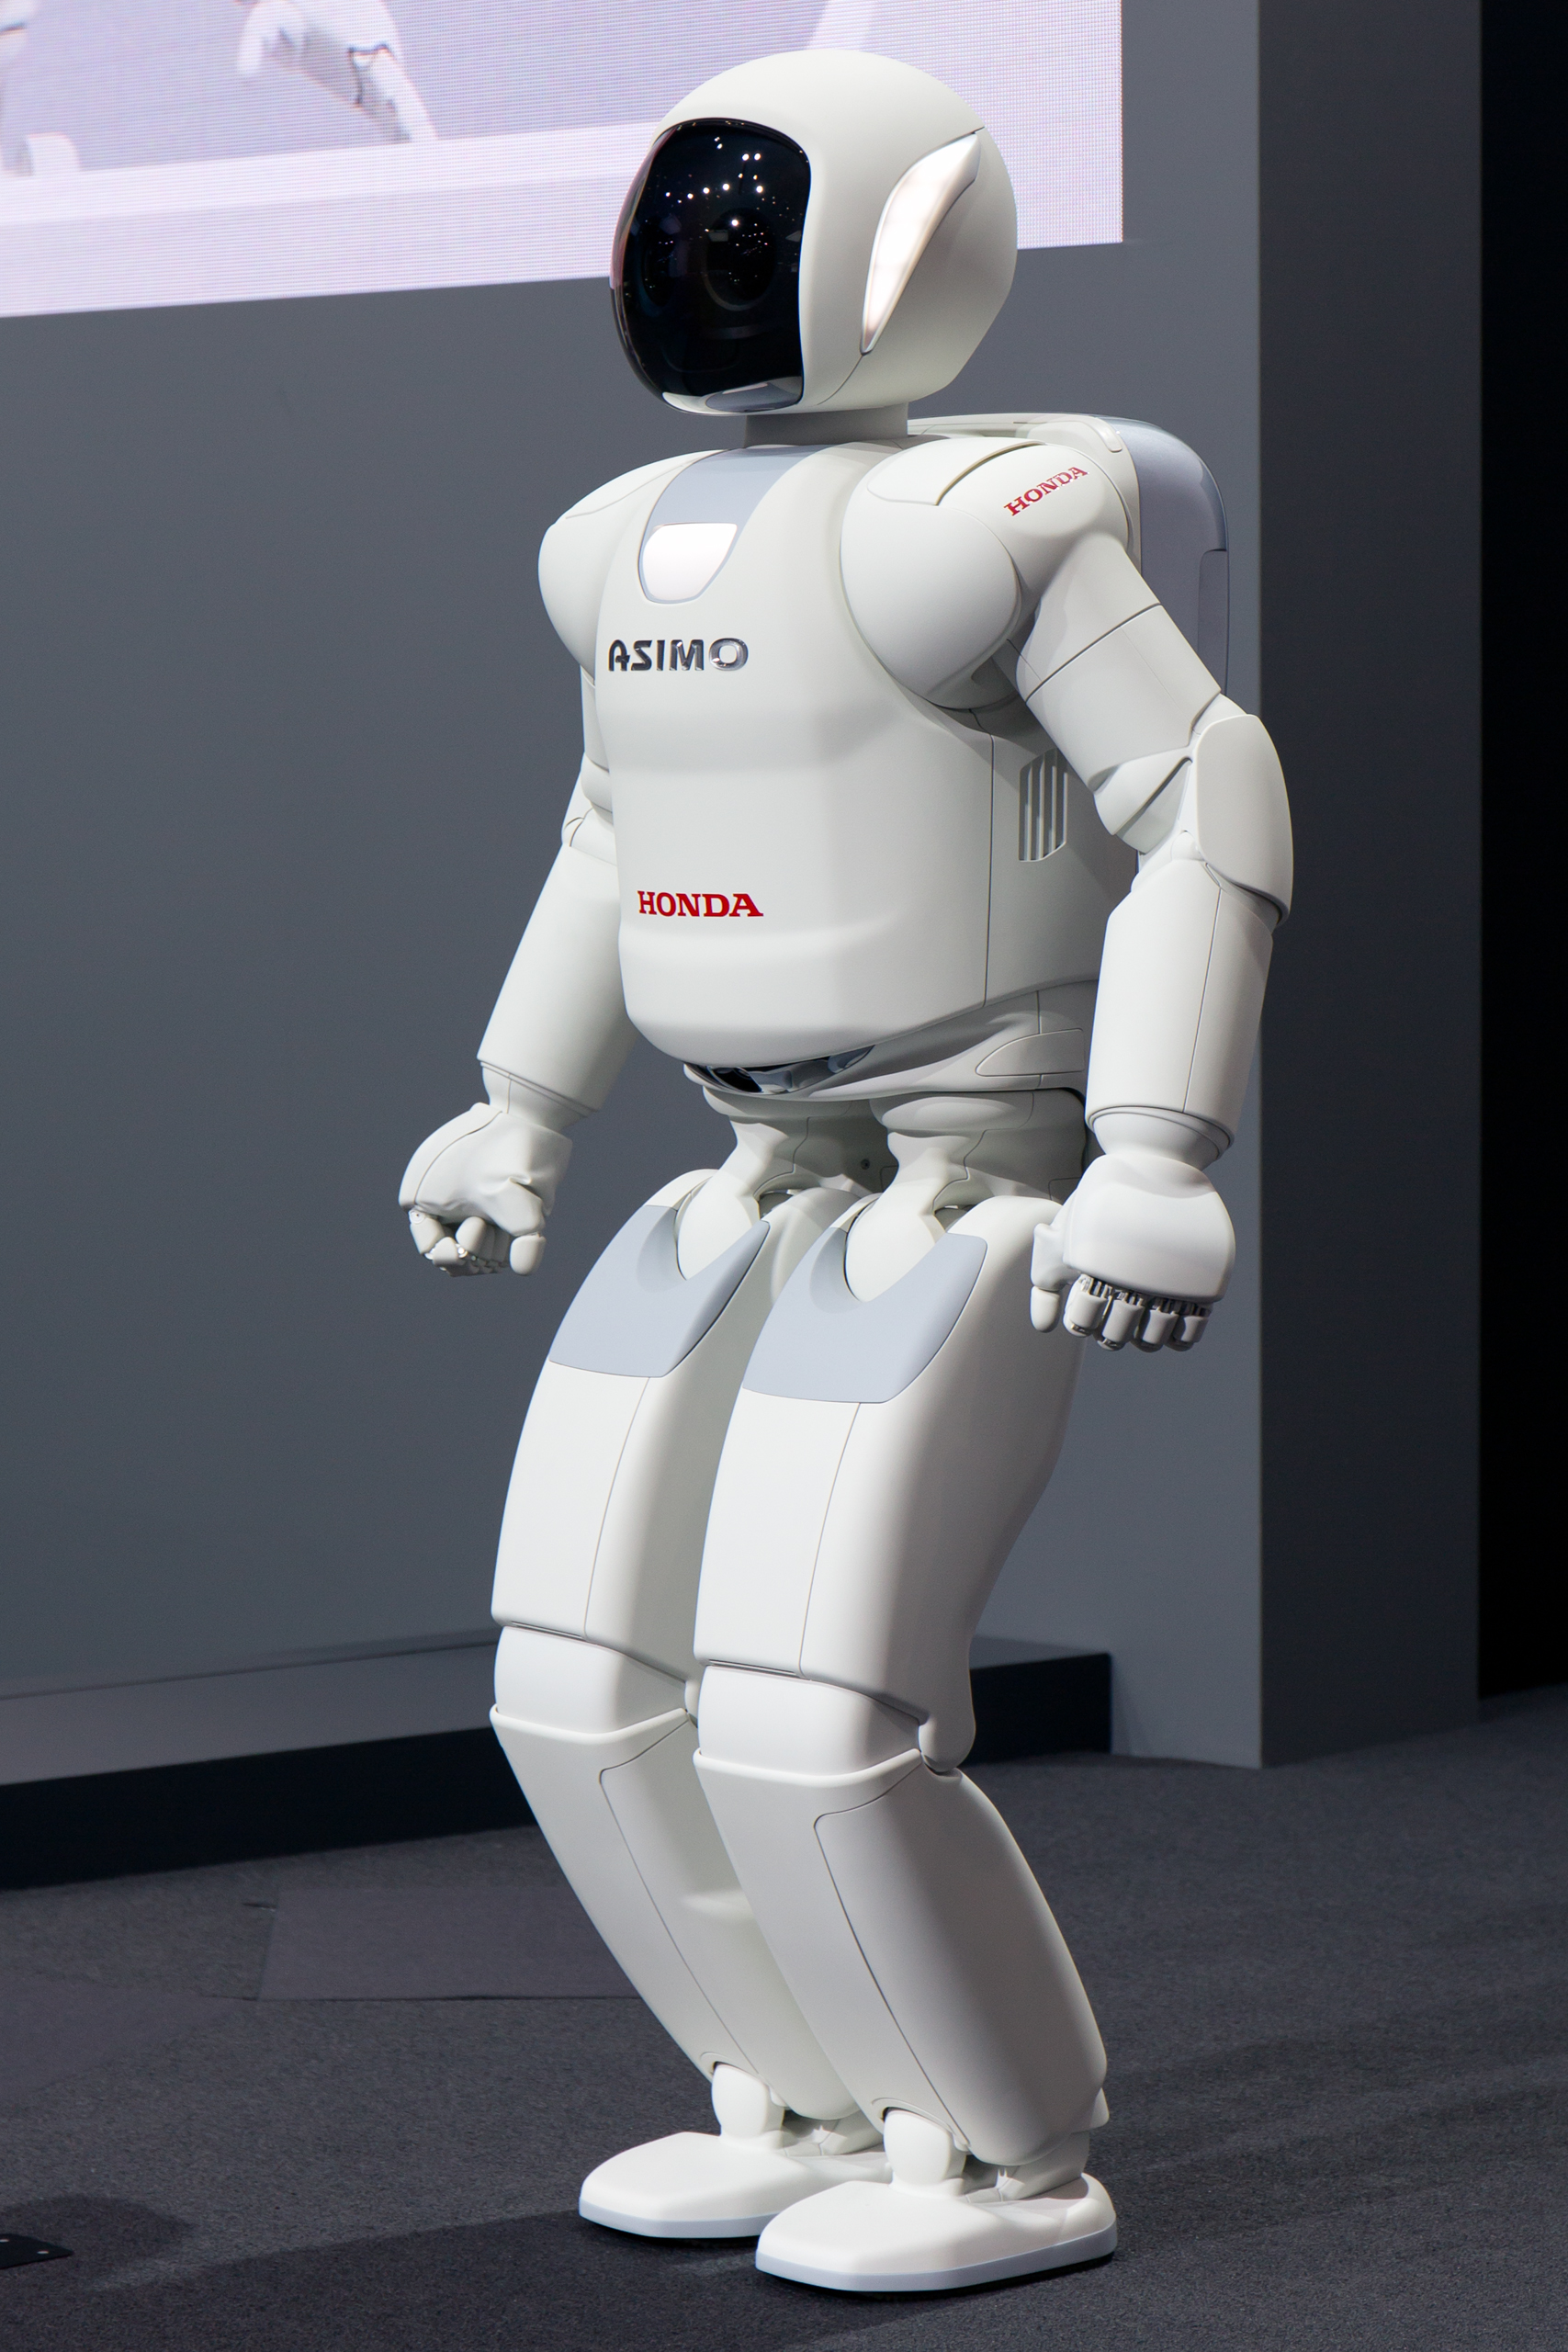
\includegraphics[width=\linewidth]{asimo}
        \caption{Honda's Asimo Robot uses position control and statically stable
        gaits. Photo by
        \href{http://commons.wikimedia.org/wiki/User:Morio}{Morio} - Own work,
        \href{http://creativecommons.org/licenses/by-sa/3.0}{CC BY-SA 3.0},
        \href{https://commons.wikimedia.org/w/index.php?curid=29969316}{Link}.}
        \label{fig:asimo}
    \end{marginfigure}

    \item\label{chal:adaptability} \emph{Prosthesis control must automatically
    adapt to novel gait situations}~~Throughout a typical day of walking, the
    amputee will adapt their gait in numerous ways, including changing speed,
    walking on slopes, walking with loads, and responding to disturbances.
    Humanoid walking controllers such as those used in the DARPA robotics
    challenge (DRC), can explicitly deal with these situations through
    centralized controllers that use the full state of the robot and the world,
    to plan and track a trajectories \citep{feng2015optimization,
    kuindersma2014efficiently, englsberger2014trajectory}. In contrast, it is
    unreasonable to expect that amputees will don full body sensing suits in
    order to provide a complete picture of the state of the amputee, prosthesis,
    and world. Therefore, prosthesis controllers must be able to adapt to novel
    situations through a decentralized approach that primarily uses the
    prosthesis state and minimal extra information.

    \item\label{chal:amputees_unique} \emph{Amputees are unique}~~Finally, we
    should be able to adapt robotic prosthesis controllers to each amputee's
    individual needs. The variation in amputee needs arise from a number of
    factors including, but not limited to, the amputee's height, weight,
    strength, endurance, reason for amputation, time since amputation,
    experience, and personal preferences. Consequently, prostheses and
    controllers should be optimized to suit individual users.
\end{challenges}

\begin{fullwidth} 
\emph{This thesis investigates a dynamic, decentralized control for transfemoral
prostheses, along with methods to optimize its parameters for individual
amputees, in order to improve gait robustness and naturalness.} 
\end{fullwidth}

\section{Approach}\label{sec:intro_approach}

We seek to improve amputee gait robustness and naturalness by employing an
alternative approach to joint control in prostheses that seeks to mimic the
underlying dynamics and control of the human neuromuscular system. In this
approach, instead of replicating recorded torque profiles with quasi-stiffness
functions, we model the dynamical system, consisting of virtual muscles and
local reflex feedback pathways, that generate joint torques during locomotion.
Crucially, the resulting prosthesis control addresses \cref{chal:dynamic} as the
virtual muscles integrate the sensed kinematic state of the prosthesis in order
to generate desired torques, not positions, at the joints. These torques, along
with the reaction forces in the amputee's socket and on the ground shape the
motion of the amputee-prosthesis system.

Moreover, prior work on neuromuscular models shows they can produce robust and
adaptable gaits. Therefore, this control approach may help address
\cref{chal:adaptability}. For example, using a neuromuscular model, an optimized
simulated biped model walked on unseen, uneven terrain with sudden drops and
steps up to 14 centimeters \citep{song2015neural}. In addition,
\citet{eilenberg2010control} successfully applied the neuromuscular control
approach to a powered ankle prosthesis, which mimics the kinematics and kinetics
of the ankle joint in human walking including its adaptation to sloped
environments.  It remains unclear, however, whether the approach and observed
adaptability extend to transfemoral prostheses with both knee and ankle joints.

To motivate our specific choice of neuromuscular control for improving amputee
gait stability, in completed work, we construct a simulation of the
amputee-prosthesis system and compare the gait robustness achieved by
neuromuscular control versus the established impedance control method. We find
that neuromuscular control enables the simulated amputee to walk further over
rougher terrain than does impedance control.

Next, to test the feasibility of controlling a real prosthesis with a
neuromuscular model, we design and build a partial powered transfemoral
prosthesis prototype with an active knee actuator and a passive, spring-loaded
ankle. The prosthesis prototype uses series elastic
actuation~\citep{pratt1995series} that allows it to accurately achieve the
torques commanded by the neuromuscular model. Initial tests with an intact user
wearing the prosthesis through an amputee simulator adaptor show that the
proposed neuromuscular control, when applied to the knee of an active
prosthesis, produce reasonable kinematics and joint torques. This positive
result motivates continued development of the prosthesis into a full active knee
and ankle transfemoral prosthesis and implementation of testing of the full
neuromuscular prosthesis control. Specifically, we plan to evaluate the
control's ability to generalize to changes in speed, incline, and disturbances
applied to the amputee.

To address the \cref{chal:amputees_unique}, we propose to optimize prosthesis
controls for specific subjects. To this end, in completed work, we develop an
algorithm that optimizes control parameters by querying users to provide
preference feedback between parameters. We test the method on problems of
increasing relevance: first by optimizing synthetic reward functions, then
optimizing the parameters of simulated dynamical systems, and finally by
optimizing neuromuscular control parameters for intact users wearing the
prosthesis through an amputee emulator brace. The results suggest the proposed
optimization method outperforms baseline methods for optimizing from user
preferences. However, we also find that pair-wise feedback is overly limiting
and that it is important to consider time adaptation. Therefore, we intend to
further develop the method to incorporate more varied forms of qualitative
feedback and to explicitly consider user adaptation over time.

Last, we seek to improve the capability of the transfemoral prosthesis to
respond to trips, which pose a significant and impactful threat to amputee
quality of life. To accomplish this goal, we propose to use imitation learning
techniques \citep{argall2009survey} to learn polices that allow the prosthesis
to appropriately respond to disturbances during swing.  The proposed method to
learn these policies will address \crefrange{chal:dynamic}{chal:amputees_unique}
in that it will be a decentralized control that only uses information from the
prosthesis and will be dynamic and personalized by working with each amputee'
innate trip response reflexes.

Previous work in this area has trained classifiers on data obtained by tripping
healthy human subjects~\citep{lawson2010stumble, shirota2014recovery}. The
authors then evaluate these classifiers via cross validation, in which a subset
of the training data is set aside and used for testing, and report low
error-rates.  However, to date no one has applied a trip classifier to
prosthesis hardware in order to initiate a trip recovery controller. Trivial
application of classifiers trained on healthy human subject data likely will
yield poor results, as the distribution of data at test time generated by a
prosthesis that is controlled by a learned policy will differ from the data used
to train that policy. The training and test time distribution mismatch violates
the i.i.d. (independent and identically drawn) assumption that
underpins classification performance. To remedy this problem, we intend to
employ the DAGGER training method \citep{ross2011reduction} that aligns the
train and test time distributions through an iterative procedure. We will
collect training and testing data to learn and evaluate the trip recovery
policies using the Push Bot robot which can apply tripping forces to subjects
via actuated tethers \citep{emanuel2016disturbance}.

\section{Expected Contributions}\label{sec:intro_contributions}

Work presented in this thesis will advance the state of the art for robotic
transfemoral prosthesis control and optimization. There are four main expected 
contributions: 

\begin{contributions}
    \item\label{contrib:pros_design} \emph{A series elastic prosthesis
    design}~~We present the design of a transfemoral prosthesis featuring series
    elastic actuators (SEAs) capable of accurately producing the torques
    commanded by the neuromuscular model, generating enough torque and speed to
    enable trip recovery experiments, and handling the impact loads expected
    during trip recovery experiments. We have made significant progress towards
    this contribution already by completing the design, manufacturing, assembly,
    and initial testing of the prosthesis' knee joint as well as the design and
    fabrication of its ankle joint.  \Cref{fig:prosthesis_design} shows the
    current stage of the prosthesis prototype with the completed SEA knee and a
    passive spring-loaded ankle well as a CAD render of the expected completed
    prosthesis design. We plan to characterize prosthesis performance in terms
    of closed-loop torque tracking bandwidth, step response, and zero torque
    tracking accuracy.
    \begin{marginfigure}[1in]
        \centering
        \includegraphics[width=\linewidth]{current_final_design}
        \caption{(a) Current stage of the prosthesis design with active knee and
        passive ankle. (b) Final design with active knee and ankle joints.}
        \label{fig:prosthesis_design}
    \end{marginfigure}

    \item\label{contrib:neuromuc_eval} \emph{Evaluation of neuromuscular
    transfemoral prosthesis control}~~We will implement the proposed
    neuromuscular prosthesis control on the SEA transfemoral prosthesis, and
    evaluate the prosthesis' ability to produce a natural and robust gait. We
    will measure nominal gait characteristics in terms of joint kinematics and
    kinetics and will present results relative to typical non-amputee gait and
    the amputee's gait using his or her prescribed prosthesis. We will also
    evaluate the ability of the control to adapt to novel circumstances such as
    changes in gait speed, ground slope, and disturbances such as sudden
    treadmill speed changes and impulses to the amputee's hip.

    \item\label{contrib:pref_opt} \emph{A method for optimizing systems via
    qualitative feedback}~~ Towards this contribution, we have developed a new
    algorithm for optimizing systems, such as prostheses, via user preferences.
    The algorithm uses preferences between pairs of control parameters to
    circumvent having to define or learn an explicit reward function for each
    user. Additionally, the algorithm employs Bayesian optimization techniques
    in order to query users for preferences that are expected to maximally
    reduce the uncertainty of the location of the optimum parameters. We will
    expand on this system to allow users to provide more forms of qualitative
    feedback such as absolute good/bad ratings, perceived ambiguity between
    parameters, and ``best so far'' statements and to explicitly consider the
    users adaptation to the prosthesis over time.

    \item\label{contrib:trip_recovery} \emph{Learning and evaluation of trip
    recovery policies}~~The last contribution is a method to learn and
    evaluation of trip response policies to recover from disturbances during
    swing. The learned policies will advance the state-of-the-art as they will
    be the first trip recovery policies implemented on prosthesis hardware,
    whereas previous policies were trained and tested offline using data
    collected from non-amputee subjects.
\end{contributions}
